\chapter{Introducci\'on} % (fold)
\label{cha:introduccion}

El presente proyecto consiste en el desarrollo de una aplicación móvil que
permita ubicar y encontrar una locación dentro del campus de la UMSS,
la aplicación deberá localizar la ubicación actual del usuario y permitir
especificar un punto de destino, mostrando a continuación el camino más corto
para llegar a destino.\\


El campus universitario abarca más de 214.000 m2 y encierra varias facultades y
oficinas administrativas, para estudiantes nuevos y antiguos o personas que
necesitan hacer trámites administrativos, incluso si solo se quiere conocer el
campus, es necesario contar con un mapa donde ubicarse.\\


Las aplicaciones móviles tienen una gran demanda por parte de la población ya
que la gran mayoría posee un smartphone o teléfono inteligente con capacidad de
ejecutar aplicaciones muy fácilmente, los smartphones cuenta también con GPS,
el cual se usa para conocer la ubicación del usuario con un margen de error de
3 metros, usando puntos de referencia geo-localizados se puede determinar la
ruta óptima para llegar a destino.\\


Es una desventaja para nuestra Universidad que no exista información confiable
de fácil acceso para poder desplazarse por el campus.\\

  \section{Antecedentes} % (fold)
  \label{sec:antecedentes}
  Actualmente Google Maps ofrece una solución a este problema pero lo ofrecen
  para las ciudades pero dentro del campus de la UMSS, google no cuenta
  información interna de la UMSS.\\


  Existen blogs o aplicaciones con Información acerca de lugares turísticos o
  de interés para visitar en nuestra ciudad como ser TripAdvisor, pero estas
  aplicaciones tampoco cuentan con información interna de la UMSS.\\


  \section{Descripción del problema} % (fold)
  \label{sec:desc_probl}
  La Universidad Mayor de San Simón no cuenta con un mapa interactivo que
  muestre la ubicación de los puntos o lugares que se encuentran dentro del
  campus universitario, este mapa sería de gran ayuda para desplazarse dentro
  del campus universitario, la falta de un mapa con estas características
  genera malestar entre la estudiantes o personas que quieren realizar trámites
  administrativos, ya que al no contar con una aplicación que muestre los puntos de interés  geolocalizados se pierde tiempo al tratar de encontrarlos.

  % \begin{figure}[!hbp]
  %   \centering
  %   \includesvg{arbolProblemas}
  %   \caption{Diagrama Arbol de Problemas}
  %   \label{fig:arbolProblemas}
  % \end{figure}


  \begin{figure}[!hbp]
    \begin{center}
      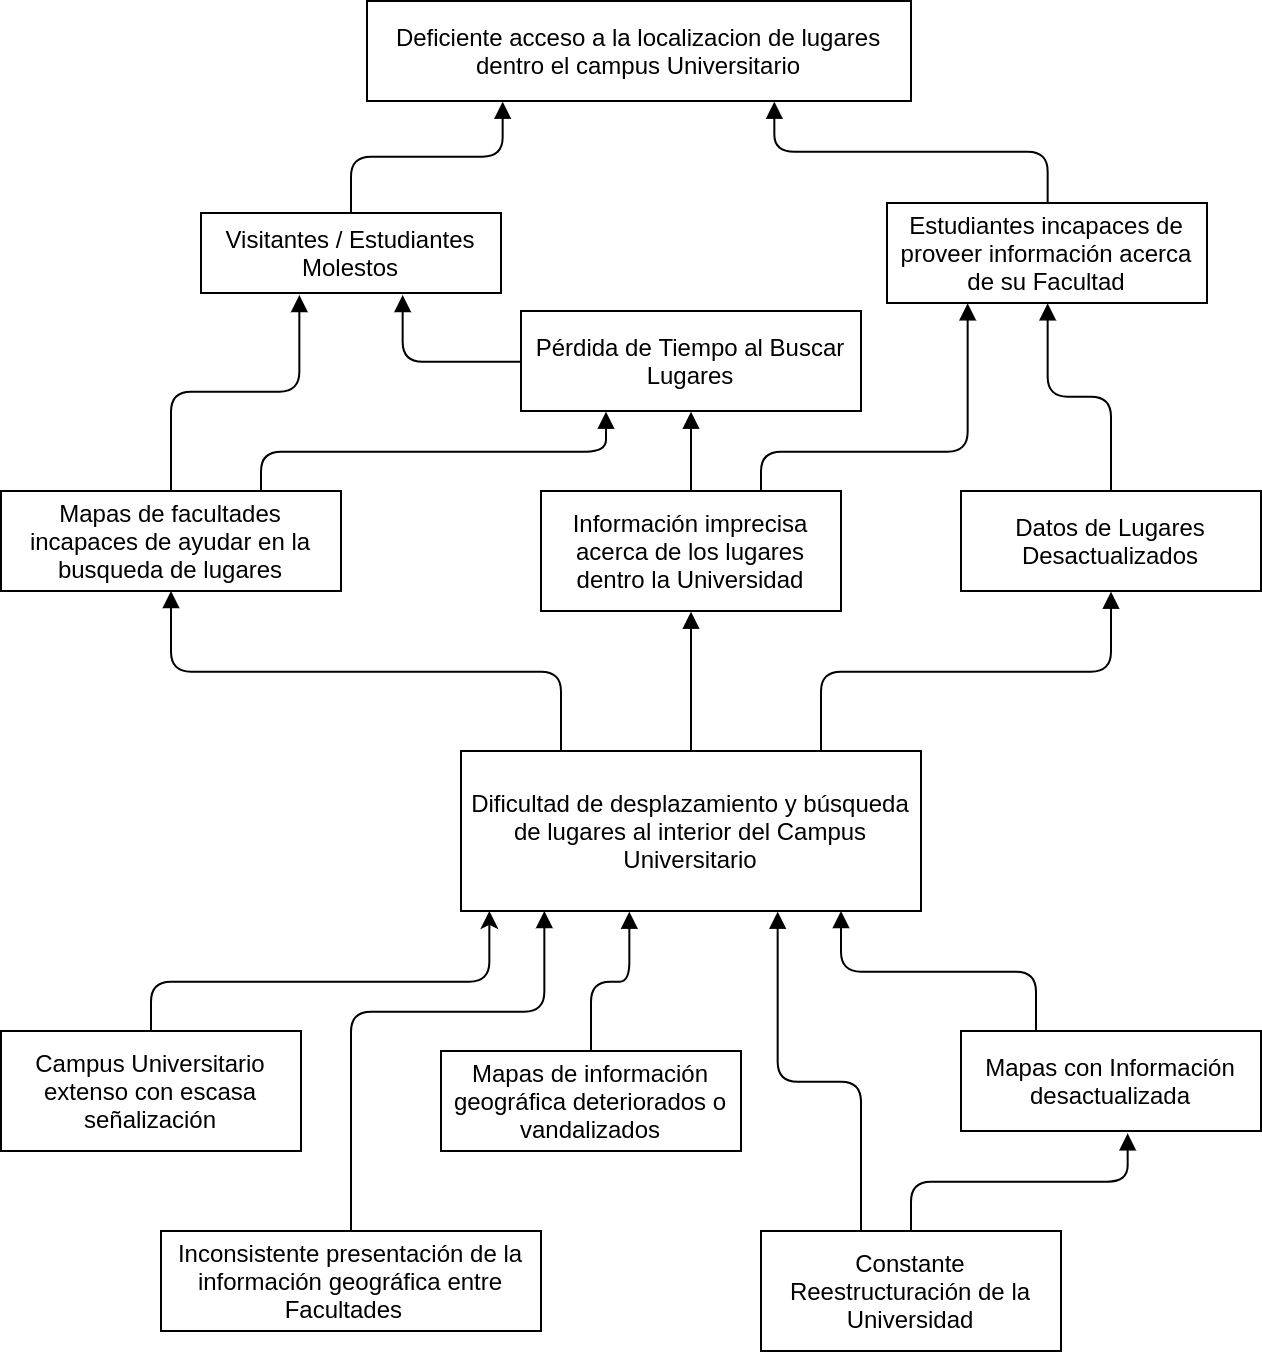
\includegraphics[width=1\textwidth]{arbolProblemas}
    \end{center}
    \caption{Diagrama Arbol de Problemas}
    \label{fig:arbolProblemas}
  \end{figure}

  \section{Objetivo general} % (fold)
  \label{sec:objetivo_general}
    \begin{quote}
      Desarrollar una aplicación web móvil responsive para optimizar la ubicación de lugares y el  Desplazamiento al interior del Campus Universitario de la Universidad Mayor de San Simon.
    \end{quote}
  % section objetivo_general (end)


  \section{Objetivos Específicos} % (fold)
  \label{sec:obj_especificos}
    \begin{itemize}
      \item Gestionar lugares geolocalizados dentro del campus Universitario.
      \item Permitir encontrar lugares dentro el campus.
      \item Priorizar lugares visitados.
      \item Generar mapa geolocalizado.
      \item Gestionar usuarios.
    \end{itemize}
  % section obj_especificos (end)


  \section{Justificación:} % (fold)
  \label{sec:justificacion}
  El Campus Universitario es bastante extenso y está en constante reestructuración, cada vez hay más aulas, las oficinas se mueven de lugar, etc. gracias a esto es que los mapas, que son escasos y están impresos sobre banners estáticos, son difíciles de actualizar. Este hecho genera malestar en estudiantes que llegan tarde a sus clases o personas que necesitan hacer trámites administrativos y no encuentran con facilidad las oficinas a las que necesitan llegar.\\


  Una aplicación que permita ubicar y encontrar locaciones además de proveer la ruta óptima dentro del campus de la Universidad Mayor de San Simón es de gran importancia para mejorar nuestra presentación a cualquier persona que necesite desplazarse por el campus Universitario.\\


  Las Aplicaciones móviles y/o web demostraron ser el futuro del desarrollo de software y la gran mayoría de los países en el mundo consumen estas soluciones y nosotros necesitamos apuntar a esta tendencia.\\
  % section justificacion (end)
% chapter introduccion (end)









% Metodología:
% Agile Unified Process (AUP) es una versión simplificada de Rational  Proceso
% Unificado  (RUP).

% Fases del ciclo de desarrollo
%   Principio: El objetivo es  identificar el alcance inicial del proyecto y una
%   arquitectura potencial del sistema.

%   Elaboración: El objetivo es confirmar la idoneidad de la arquitectura del sistema.
%   Construcción: El objetivo es desarrollar software funcional dentro de un sistema regular e incremental periódicamente que mire las necesidades de las partes interesadas.
%   Transición: El objetivo es validar y desplegar el sistema en su entorno de producción.
% Las disciplinas del ciclo de desarrollo se llevan de manera iterativa y son
% las siguientes
%   Modelo: El objetivo de esta disciplina es entender el negocio de la organización, el dominio del problema que se ocupa el proyecto, y determinar una solución viable para hacer frente al dominio del problema.
%   Aplicación: El objetivo de esta disciplina es transformar el modelo de su (s) en el código ejecutable y para llevar a cabo un nivel básico de las pruebas, en las pruebas de unidad en particular.
%   Prueba: El objetivo de esta disciplina consiste en realizar una evaluación objetiva para asegurar la calidad. Esto incluye encontrar defectos, validar que el sistema funcione como está previsto, y verificar que se cumplan los requisitos.
%   Implementación: El objetivo de esta disciplina es el plan para la entrega del sistema y para ejecutar el plan para que el sistema a disposición de los usuarios finales.
%   Gestión de la Configuración: El objetivo de esta disciplina consiste en administrar el acceso a artefactos de su proyecto. Esto incluye no sólo el seguimiento de versiones de los artefactos a través del tiempo, sino también el control y la gestión de los cambios a los mismos.
%   Gestión de Proyectos: El objetivo de esta disciplina es dirigir las actividades que lleva a cabo en el proyecto. Esto incluye la gestión de riesgos, la dirección de personas (la asignación de tareas, seguimiento de los progresos, etc.), y coordinar con la gente y los sistemas fuera del alcance del proyecto para asegurarse de que se entregue a tiempo y dentro del presupuesto.
%   Para el Medio Ambiente: El objetivo de esta disciplina es apoyar el resto de los esfuerzos por garantizar que el proceso, la orientación adecuada (las normas y directrices), y herramientas (hardware, software, etc.) están disponibles para el equipo según sea necesario.
% % Fig. Ciclo de vida del Proceso Unificado Ágil
